\chapter{Demonstrating the Monitor in Action}
\label{chap:MonitorInAction}

In this chapter we present the culmination of our efforts with a demonstration of the monitor detecting a collusion attack.

\section{Installation}

\begin{wrapfigure}[15]{r}{0.44\linewidth}
	\centering
	\vspace{-12pt}
	\includegraphics[height=0.39\textheight]{graphics/PhonePhotos/01 - Installation.jpg}
	\caption{Monitor Installed}
	\label{fig:MonitorInstalled}
\end{wrapfigure}

To demonstrate the monitor in action it is necessary to stage collusion attacks at will.  We used the reader and publisher applications that we developed earlier to perform the attack.  They were both installed onto a rooted Motorola G4 Play phone running Android 6.0.1, along with the interceptor module and the monitor.  Figure \ref{fig:MonitorInstalled} shows the installation.  We also added two contacts to the phone's contact list, shown in figure \ref{fig:DisplayingContacts}.

\section{Before Collusion}

Figure \ref{fig:BeforeCollusion} shows the state of the phone before the attack.  The publisher in figure \ref{fig:PublisherBefore} is ready to receive contacts.  The monitor is active in figure \ref{fig:MonitorBefore} but has not yet detected collusion.\\

\begin{figure}[h!]
	\centering
	\begin{subfigure}{0.49\textwidth}
	  \centering
      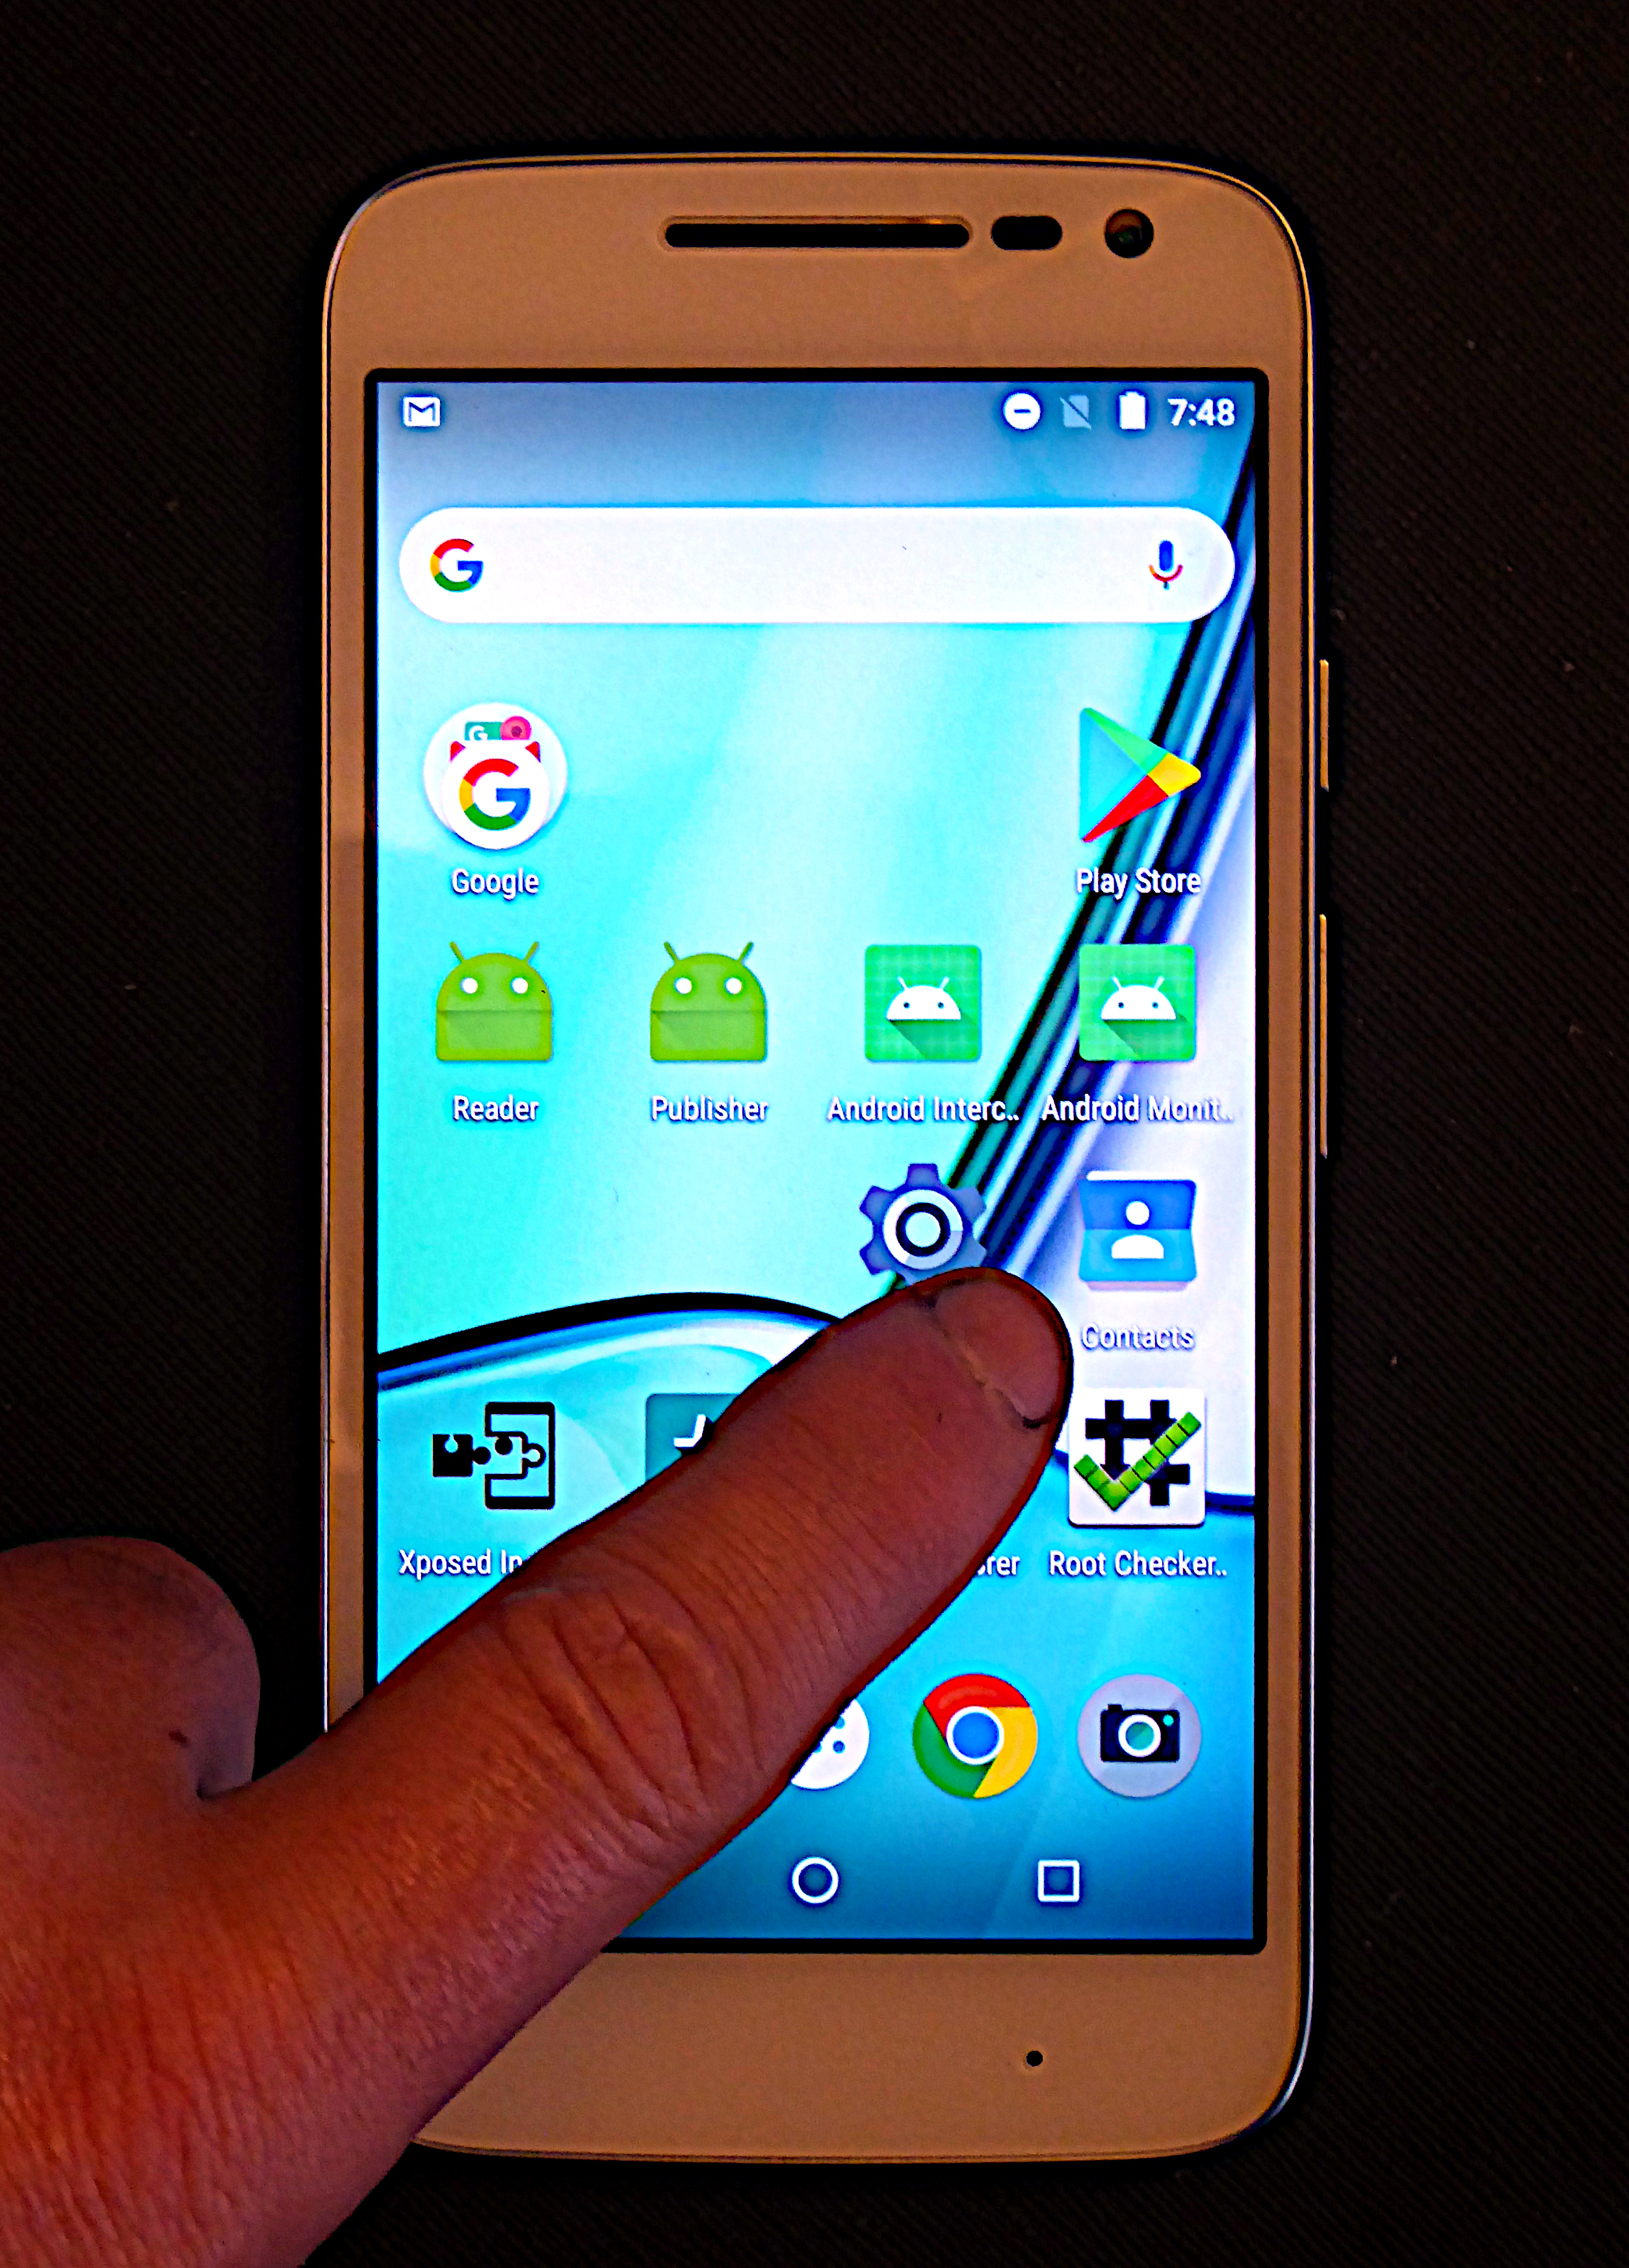
\includegraphics[height=0.45\textheight]{graphics/PhonePhotos/02 - BringUpContacts.jpg}
      \caption{Opening the Contacts List}
      \label{fig:OpeningContacts}
	\end{subfigure}
\hfill	
	\begin{subfigure}{0.49\textwidth}
		\centering
        \includegraphics[height=0.45\textheight]{graphics/PhonePhotos/03 - DisplayContacts.jpg}
        \caption{Displaying the Contacts}
        \label{fig:DisplayingContacts}
	\end{subfigure}
	\caption{Stored Contacts List}
	\label{fig:ContactsList}
\end{figure}

We started the collusion attack manually by telling the reader app to send the contacts.  Figure \ref{fig:ReaderSend} shows us sending the contacts list by pressing the send button on the reader.  The publisher app completed the attack when it received the contacts and displayed them on the screen.  We can see in figure \ref{fig:PublisherAfter} that this happened because the publisher log confirms it received two contacts, identical to those displayed on the reader app.  And we can see it has put them on the screen.

\section{After Collusion}

While the attack was in progress, the interceptor module intercepted the operating system calls used to perform the attack and informed the monitor by sending it trace events.  The monitor writes a log entry for every event it receives and entries for the trace evaluation result.  Figure \ref{fig:MonitorAfter} shows the monitor application and the log it generated during the attack.  

The log entry highlighted by the red rectangle is an alert that indicates the monitor has successfully detected a complete attack sequence.  The log entries immediately before the alert show the complete attack sequence (q,s,r,p) and the log entries immediately after the alert list the trace events that caused the monitor to be triggered.

\newpage

\begin{figure}[H]
	\centering
	\begin{subfigure}{0.49\textwidth}
		\centering
		\includegraphics[height=0.45\textheight]{graphics/PhonePhotos/05 - PublisherBefore.jpg}
		\caption{Publisher Before Collusion}
		\label{fig:PublisherBefore}
	\end{subfigure}
\hfill	
	\begin{subfigure}{0.49\textwidth}
		\centering
		\includegraphics[height=0.45\textheight]{graphics/PhonePhotos/06 - MonitorBefore.jpg}
		\caption{Monitor Before Collusion}
		\label{fig:MonitorBefore}
	\end{subfigure}
\\
	\begin{subfigure}{0.49\textwidth}
		\centering
		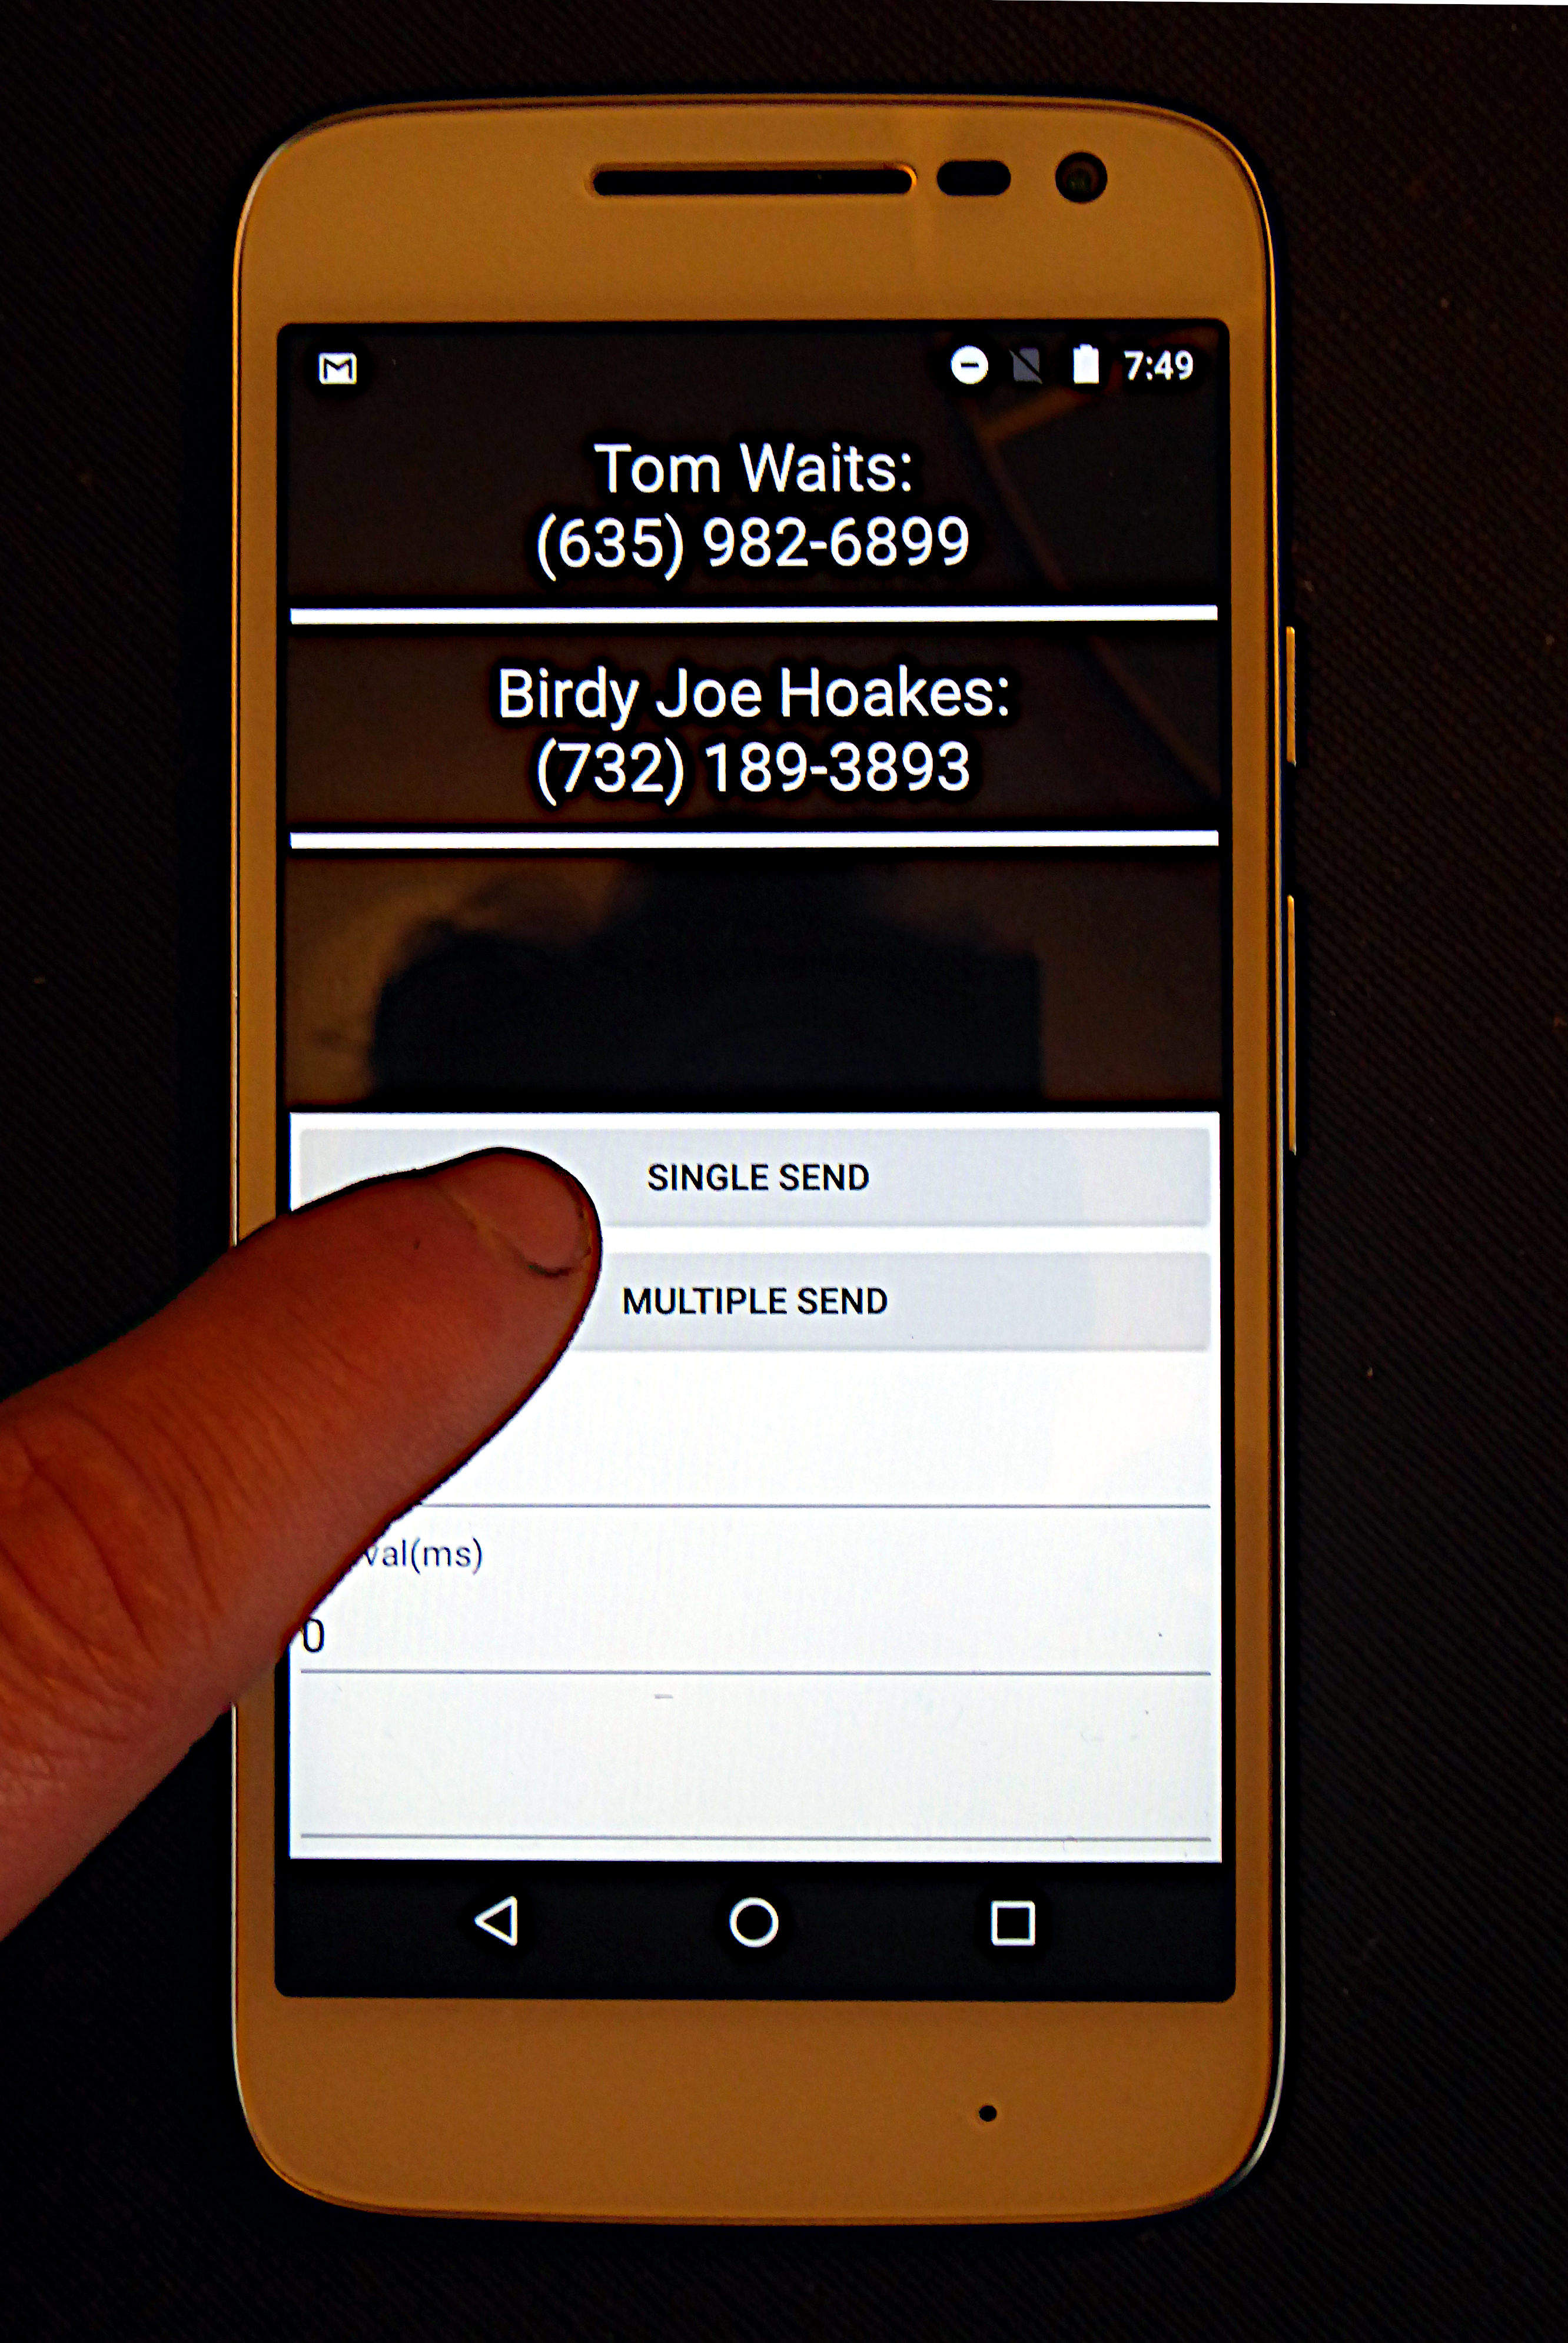
\includegraphics[height=0.45\textheight]{graphics/PhonePhotos/07 - ReaderSend.jpg}
		\caption{Reader Sending Contacts}
		\label{fig:ReaderSend}
	\end{subfigure}
	\caption{Before Collusion}
	\label{fig:BeforeCollusion}
\end{figure}

\newpage

\begin{figure}[h!]
	\centering
	\includegraphics[width=0.7\linewidth]{graphics/PhonePhotos/08 - PublisherAfter.jpg}
	\caption{Publisher After Collusion}
	\label{fig:PublisherAfter}
\end{figure}

\newpage

\begin{figure}[h!]
   \centering
   \includegraphics[width=0.7\linewidth]{graphics/PhonePhotos/09 - MonitorAfter.jpg}
   \caption{Monitor After Collusion}
   \label{fig:MonitorAfter}
\end{figure}

\newpage

\section{Negative Demonstration}

To illustrate the monitor operating among benign applications, we performed the same demonstration again but, the reader application was modified to not send the contacts it queried.  Doing this breaks the sequence of events required for a collusion attack because the reader will do nothing more than look at the contacts list.

\begin{wrapfigure}[26]{l}{0.6\linewidth}
	\centering
	\vspace{-12pt}
	\includegraphics[width=0.58\textwidth]{graphics/PhonePhotos/10 - NegativeTest.jpg}
	\caption{Negative Demonstration}
	\label{fig:NegativeDemonstration}
\end{wrapfigure}

For brevity, figure \ref{fig:NegativeDemonstration} shows only the monitor after the demonstration.  In the log, it can be seen that query and publish events both occurred, but there is no send event and, therefore, no receive.  The reader might be asking how did the monitor receive a publish event when the publisher app did not receive any contacts?  The log reveals the answer:  The publish event received by the monitor was performed by the reader application.  What happened is that after querying the contacts, the reader app displayed them on the screen.  It called the same method that the publisher app uses to display the contacts, thus, the interceptor noticed this and publish event was generated.  

Although the monitor received an event to say the publish event occurred, neither the static, nor dynamic conditions were met.  Therefore, collusion was not detected.